\documentclass[journal, 11pt, onecolumn]{IEEEtran}
\usepackage{graphicx}
\usepackage{fancyhdr}
\usepackage{lastpage}
\usepackage[a4paper,margin=1in]{geometry}
\usepackage{newtxtext,newtxmath}
\usepackage{enumitem}
\usepackage{multicol}
\usepackage{array}

\usepackage{cite}
\usepackage{amsmath,amssymb,amsfonts,amsthm}
\usepackage{algorithmic}
\usepackage{graphicx}
\usepackage{textcomp}
\usepackage{xcolor}

\usepackage{listings}
\usepackage{enumitem}
\usepackage{mathtools}
\usepackage{gensymb}
\usepackage{comment}
\usepackage[breaklinks=true]{hyperref}
\usepackage{tkz-euclide} 
\usepackage{gvv}                                        
%\def\inputGnumericTable{}                                 
\usepackage[latin1]{inputenc}     
\usepackage{xparse}
\usepackage{color}                                            
\usepackage{array}                                            
\usepackage{longtable}                                       
\usepackage{calc}                                             
\usepackage{multirow}
\usepackage{multicol}
\usepackage{hhline}                                           
\usepackage{ifthen}                                           
\usepackage{lscape}
\usepackage{tabularx}
\usepackage{array}
\usepackage{float}
\newtheorem{theorem}{Theorem}[section]
\newtheorem{problem}{Problem}
\newtheorem{proposition}{Proposition}[section]
\newtheorem{lemma}{Lemma}[section]
\newtheorem{corollary}[theorem]{Corollary}
\newtheorem{example}{Example}[section]
\newtheorem{definition}[problem]{Definition}
\newcommand{\BEQA}{\begin{eqnarray}}
\newcommand{\EEQA}{\end{eqnarray}}
\newcommand{\define}{\stackrel{\triangle}{=}}
\theoremstyle{remark}
\newtheorem{rem}{Remark}

\graphicspath{{figs/}}


\pagestyle{fancy}

% Header and footer text
\fancyhead[L]{2020}
\fancyhead[C]{}
\fancyhead[R]{MAIN PAPER-MT}
\fancyfoot[L]{MT}
\fancyfoot[C]{}
\fancyfoot[R]{\thepage/\pageref{LastPage}}

% Adjust distances
\setlength{\headheight}{14pt}
\setlength{\headsep}{5pt}
\setlength{\footskip}{20pt}


% Line thickness
\renewcommand{\headrulewidth}{0.4pt}
\renewcommand{\footrulewidth}{0.4pt}

\begin{document}

\begin{center}
    \Large{AI25btech11038}
\end{center} 

\begin{enumerate}

\item He is known for his unscrupulous ways. He always sheds \_\_\_ tears to deceive people
\begin{multicols}{4}
\begin{enumerate}
    \item fox\textquotesingle s
    \item crocodile\textquotesingle s
    \item crocodile
    \item fox
\end{enumerate}
\end{multicols}
\hfill(GATE MT 2020)

\item Jofra Archer, the England fast bowler, is \_\_\_ than accurate.
\begin{multicols}{4}
\begin{enumerate}
    \item more fast 
    \item faster
    \item less fast
    \item more faster
\end{enumerate}
\end{multicols}
\hfill(GATE MT 2020)

\item Select the word that fits the analogy: 
\begin{align}
    Build: Building :: Grow: \_\_\_
\end{align}
\begin{multicols}{4}
\begin{enumerate}
    \item Grown 
    \item Grew
    \item Growed
    \item Growing
\end{enumerate}
\end{multicols}
\hfill(GATE MT 2020)

\item I do not think you know the case well enough to have opinions. Having said that, I agree with your other point.\\
What does the phrase "having said that" mean in the given text?
\begin{multicols}{2}
\begin{enumerate}
    \item as opposed to what I have said 
    \item despite what I have said
    \item in addition to what I have said
    \item contrary to what I have said
\end{enumerate}
\end{multicols}
\hfill(GATE MT 2020)

\item Define \sbrak{x} as the greatest integer less than or equal to $x$, for each $x \in  \brak{-\infty, \infty}$. If $y$ = \sbrak{x}, then the area under $y$ for $x \in \sbrak{1,4}$ is
\begin{multicols}{4}
\begin{enumerate}
    \item 1 
    \item 3
    \item 4
    \item 6
\end{enumerate}
\end{multicols}
\hfill(GATE MT 2020)

\item Crowd funding deals with mobilisation of funds for a project from a large number of people, who would be willing to invest smaller amounts through web-based platforms in the project.  

Based on the above paragraph, which of the following is correct about crowd funding?

\begin{multicols}{2}
\begin{enumerate}
\item Funds raised through unwilling contributions on web-based platforms.  
\item Funds raised through large contributions on web-based platforms.  
\item Funds raised through coerced contributions on web-based platforms.  
\item Funds raised through voluntary contributions on web-based platforms.  
\end{enumerate}
\end{multicols}
\hfill(GATE MT 2020)

\item P, Q, R and S are to be uniquely coded using $\alpha$ and $\beta$. If P is coded as $\alpha\alpha$ and Q as $\alpha\beta$, then R and S, respectively, can be coded as \_\_\_\_\_

\begin{multicols}{2}
\begin{enumerate}
\item $\beta\alpha$ and $\alpha\beta$  
\item $\beta\beta$ and $\alpha\alpha$  
\item $\alpha\beta$ and $\beta\beta$  
\item $\beta\alpha$ and $\beta\beta$  
\end{enumerate}
\end{multicols}
\hfill(GATE MT 2020)

\item The sum of the first $n$ terms in the sequence 8, 88, 888, 8888, $\dots$ is \_\_\_\_\_

\begin{multicols}{2}
\begin{enumerate}
\item $\dfrac{81}{80}(10^{n}-1) + \dfrac{9}{8}n$  
\item $\dfrac{81}{80}(10^{n}-1) - \dfrac{9}{8}n$  
\item $\dfrac{80}{81}(10^{n}-1) + \dfrac{8}{9}n$  
\item $\dfrac{80}{81}(10^{n}-1) - \dfrac{8}{9}n$  
\end{enumerate}
\end{multicols}
\hfill(GATE MT 2020)

\item Select the graph that schematically represents BOTH $y = x^{m}$ and $y = x^{1/m}$ properly in the interval $0 \leq x \leq 1$, for integer values of $m$, where $m > 1$.
\begin{enumerate}
\item \begin{figure}[H]
    \centering
    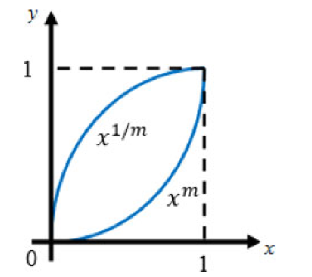
\includegraphics[width=0.25\linewidth]{figs/image1''.png}
    \caption{}
    \label{fig:placeholder}
\end{figure}  
\item \begin{figure}[H]
    \centering
    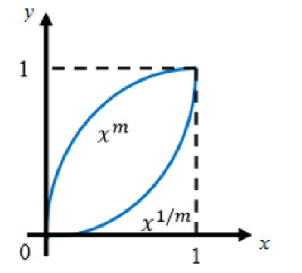
\includegraphics[width=0.25\linewidth]{figs/image2''.png}
    \caption{}
    \label{fig:placeholder}
\end{figure}  
\item \begin{figure}[H]
    \centering
    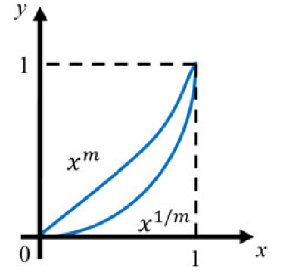
\includegraphics[width=0.25\linewidth]{figs/image3''.png}
    \caption{}
    \label{fig:placeholder}
\end{figure}    
\item \begin{figure}[H]
    \centering
    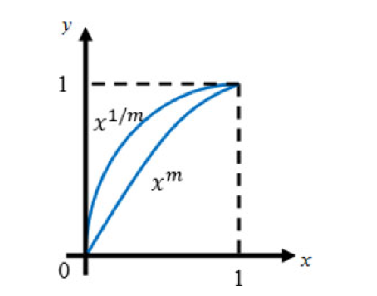
\includegraphics[width=0.25\linewidth]{figs/image4''.png}
    \caption{}
    \label{fig:placeholder}
\end{figure}      
\end{enumerate}
\hfill(GATE MT 2020)

\item The bar graph shows the data of the students who appeared and passed in an examination for four schools P, Q, R and S. The average of success rates \brak{in percentage} of these four schools is \_\_\_\_\_
\begin{figure}[H]
    \centering
    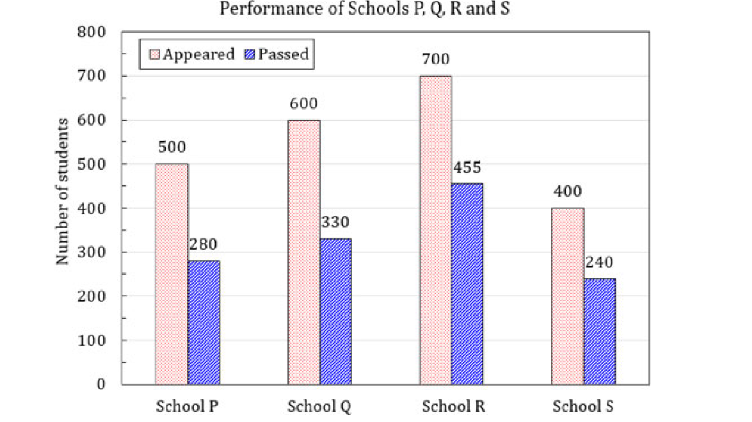
\includegraphics[width=1\linewidth]{figs/image5''.png}
    \caption{}
    \label{fig:placeholder}
\end{figure}
\begin{multicols}{4}
\begin{enumerate}
\item 58.5\%  
\item 63.7\%  
\item 45\%  
\item 23.6\%
\end{enumerate}
\end{multicols}
\hfill(GATE MT 2020)

\item The general solution to the following homogeneous ODE,  

$$
\dfrac{d^{2}y}{dt^{2}} + 4\dfrac{dy}{dt} + 3y = 0,
$$

is,  

$$
y(t) = c_{1}e^{\lambda_{1}t} + c_{2}e^{\lambda_{2}t}.
$$

The values of $\lambda_{1}$ and $\lambda_{2}$ are:  

\begin{multicols}{2}
\begin{enumerate}
\item $-1$ and $-3$  
\item $-3$ and $-3$  
\item $1$ and $-3$  
\item $1$ and $3$  
\end{enumerate}
\end{multicols}
\hfill(GATE MT 2020)

\item The number of independent elastic constants of an isotropic material is:  

\begin{multicols}{2}
\begin{enumerate}
\item $1$  
\item $2$  
\item $3$  
\item $4$  
\end{enumerate}
\end{multicols}
\hfill(GATE MT 2020)

\item A slip system consists of a slip plane and a slip direction. Which one of the following is NOT a valid slip system in a FCC copper crystal?  

\begin{multicols}{2}
\begin{enumerate}
\item $\brak{111}\sbrak{10\bar{1}}$  
\item $\brak{1\bar{1}1}\sbrak{01\bar{1}}$  
\item $\brak{\bar{1}11}\sbrak{10\bar{1}}$  
\item $\brak{1\bar{1}1}\sbrak{101}$  
\end{enumerate}
\end{multicols}
\hfill(GATE MT 2020)

\item A dielectric material is:  

\begin{multicols}{2}
\begin{enumerate}
\item Electrical conductor  
\item Metallic magnet  
\item Two coupled electrical conductors  
\item Electrical insulator  
\end{enumerate}
\end{multicols}
\hfill(GATE MT 2020)

\item Which one of the following processes is an example of an electrolytic cell?  
\begin{enumerate}
\item Corrosion of a metal rod in ambient atmosphere  
\item Charging of a rechargeable battery  
\item Discharging of a rechargeable battery  
\item Sacrificial cathodic protection system  
\end{enumerate}
\hfill(GATE MT 2020)

\item Which one of the following statements regarding selective leaching of a binary alloy is TRUE?  

\begin{multicols}{2}
\begin{enumerate}
\item The lower atomic weight element is leached.  
\item The element having higher diffusivity is leached.  
\item The more electronegative element is leached.  
\item The element with lower density is leached.  
\end{enumerate}
\end{multicols}
\hfill(GATE MT 2020)

\item In green sand casting, which one of the following is NOT a part of the gating system?  

\begin{multicols}{2}
\begin{enumerate}
\item Runner  
\item Sprue  
\item Riser  
\item Pouring basin  
\end{enumerate}
\end{multicols}
\hfill(GATE MT 2020)

\item For a material to exhibit superplasticity, one of the requirements is:  

\begin{multicols}{2}
\begin{enumerate}
\item Coarse-grained microstructure  
\item High strain-rate sensitivity  
\item Low strain-hardening exponent  
\item High modulus of elasticity  
\end{enumerate}
\end{multicols}
\hfill(GATE MT 2020)

\item The dye penetrant test for detecting flaws is based on:  

\begin{multicols}{2}
\begin{enumerate}
\item Magnetism  
\item Sound propagation  
\item X-ray absorption  
\item Capillary action  
\end{enumerate}
\end{multicols}
\hfill(GATE MT 2020)

\item When 1 mole of C$_3$H$_8$ at 300 K is burnt with stoichiometric amount of oxygen at 300 K to form CO$_2$ and H$_2$O, the adiabatic flame temperature is 5975 K. If C$_3$H$_8$ is burnt under the same conditions but with excess oxygen, the adiabatic flame temperature will be  

\begin{multicols}{2}
\begin{enumerate}
\item equal to 5975 K irrespective of the amount of excess oxygen.  
\item higher than 5975 K irrespective of the amount of excess oxygen.  
\item lower than 5975 K irrespective of the amount of excess oxygen.  
\item higher or lower than 5975 K depending on the amount of excess oxygen.  
\end{enumerate}
\end{multicols}
\hfill(GATE MT 2020)

\item Two solid spheres $X$ and $Y$ of identical diameter are made of different materials having thermal diffusivities 
$100 \times 10^{-6} \ \text{m}^2\text{s}^{-1}$ and $25 \times 10^{-6} \ \text{m}^2\text{s}^{-1}$ respectively. Both spheres are heated in a furnace maintained at $1000 \, K$. If the center of the sphere $X$ reaches $800 \, K$ in $1$ hour, time required for the center of sphere $Y$ to reach $800 \, K$ is
\begin{enumerate}
\item 1 hour.  
\item 2 hours.  
\item 4 hours.  
\item 16 hours.  
\end{enumerate}
\hfill(GATE MT 2020)


\item Select the correct spectra (shown on a log-log scale in the figures) for emission from a gray surface and a black body, both maintained at $1000 \, K$.
\begin{enumerate}
\item Figure (A)  
\item Figure (B)  
\item Figure (C)  
\item Figure (D)  
\end{enumerate}
\hfill(GATE MT 2020)


\item Given the three vectors $X = -i - j + k$, $Y = -i + 2j + k$ and $Z = i + k$, which one of the following statements is TRUE?
\begin{enumerate}
\item $X, Y$ and $Z$ are mutually perpendicular.  
\item $X, Y$ and $Z$ are coplanar.  
\item $X$ makes an angle of $30^\circ$ with the normal to the plane containing $Y$ and $Z$.  
\item $Z$ makes an angle of $60^\circ$ with the normal to the plane containing $X$ and $Y$.  
\end{enumerate}
\hfill(GATE MT 2020)


\item Angle between two neighboring tetrahedral bonds in Si having a diamond cubic structure is:
\begin{enumerate}
\item $102.5^\circ$  
\item $109.5^\circ$  
\item $120^\circ$  
\item $135.5^\circ$  
\end{enumerate}
\hfill(GATE MT 2020)


\item The sequence of precipitation during aging of Al 4 wt.\% Cu alloy is:
\begin{enumerate}
\item GP zone $\rightarrow \theta'' \rightarrow \theta' \rightarrow \theta$  
\item GP zone $\rightarrow \theta \rightarrow \theta' \rightarrow \theta''$  
\item GP zone $\rightarrow \theta' \rightarrow \theta'' \rightarrow \theta$  
\item $\theta'' \rightarrow \theta' \rightarrow$ GP zone $\rightarrow \theta$  
\end{enumerate}
\hfill(GATE MT 2020)


\item The indenter used in Rockwell hardness measurements on C scale is
\begin{enumerate}
\item diamond cone.  
\item 10 mm steel ball.  
\item diamond pyramid.  
\item 1/16-in. steel ball.  
\end{enumerate}
\hfill(GATE MT 2020)


\item For the function $y = a^x$, the derivative $\dfrac{dy}{dx}$ at $x=1$ is:
\begin{enumerate}
\item 1  
\item $a$  
\item $a^2$  
\item $a \ln a$  
\end{enumerate}
\hfill(GATE MT 2020)


\item Cupola is a furnace used to produce
\begin{enumerate}
\item cast irons.  
\item plain carbon steels.  
\item copper alloys.  
\item aluminium alloys.  
\end{enumerate}
\hfill(GATE MT 2020)


\item The functions $y = e^x$ and $y = e^{-x}$ intersect at the point:
\begin{multicols}{4}
\begin{enumerate}
\item \brak{1, 3} 
\item \brak{-2, 2}  
\item \brak{0, 1}
\item \brak{-1, -1}  
\end{enumerate}
\end{multicols}
\hfill(GATE MT 2020)


\item A heavily cold-worked metal will
\begin{enumerate}
\item have lower strength and higher ductility compared to annealed metal.  
\item have higher strength and lower ductility compared to annealed metal.  
\item have higher strength and higher ductility compared to annealed metal.  
\item have lower strength and lower ductility compared to annealed metal.  
\end{enumerate}
\hfill(GATE MT 2020)


\item For the function $f(x)$ given in the figure, the value of 
$$
\int_{0}^{1} (1 - f(x)) \, dx
$$
is \underline{\hspace{2cm}} (round off to one decimal place).  

\begin{figure}[H]
    \centering
    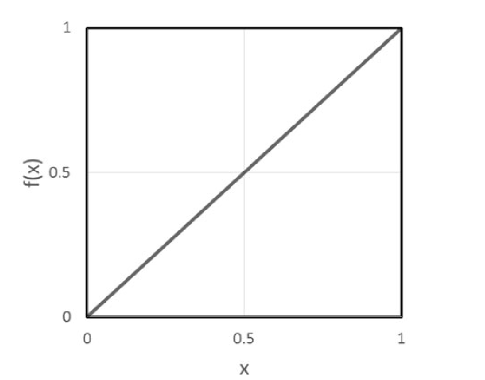
\includegraphics[width=0.5\linewidth]{figs/image6''.png}
    \caption{}
    \label{fig:placeholder}
\end{figure}
\hfill(GATE MT 2020)


\item A component subjected to tensile stress in a mechanical device is monitored periodically for cracks by NDT. The NDT technique can only detect cracks (both surface and internal) which are larger than 1 mm. Keeping a 10\% margin of safety, the maximum allowed tensile stress on the component will be \underline{\hspace{2cm}} MPa (round off to the nearest integer).  

Given, fracture toughness $K_{IC} = 30 \, \text{MPa} \, \text{m}^{1/2}$ and assume crack geometry factor of unity.
\hfill(GATE MT 2020)


\item An iron plate with a total exposed surface area of $50 \, \text{cm}^2$ undergoes atmospheric corrosion. If $200 \, g$ of weight is lost over a period of 10 years, then the corrosion rate is \underline{\hspace{2cm}} $\text{kg} \cdot \text{m}^{-2} \cdot \text{year}^{-1}$ (round off to the nearest integer).
\hfill(GATE MT 2020)


\item In cold-rolling, for the sheet to be drawn into rolls, the angle of contact (or angle of bite) should be less than or equal to \underline{\hspace{2cm}} degree (round off to one decimal place).  

Given, the coefficient of friction between sheet and roll is 0.1.
\hfill(GATE MT 2020)


\item The number of atoms per unit area in (100) plane of Pb is \underline{\hspace{2cm}} nm$^{-2}$ (round off to the nearest integer).  

Given, crystal structure and atomic radius of Pb are FCC and 0.175 nm respectively.
\hfill(GATE MT 2020)


\item In the edge dislocation configuration given in the figure, dislocations X and Y are fixed and separated by a distance $2h$ on the same slip plane. Dislocation Z is free to glide on a parallel slip plane. The two slip planes are separated by a distance $h$. Which one of the following statements is TRUE regarding the stability of dislocation Z at positions 1, 2 and 3?  

Assume all dislocations have identical Burgers vector.  

\begin{figure}[H]
    \centering
    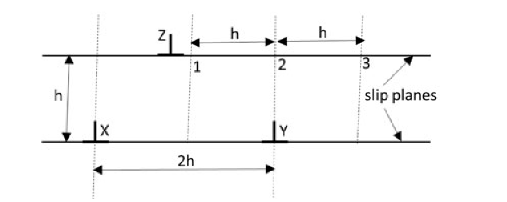
\includegraphics[width=0.5\linewidth]{figs/image7''.png}
    \caption{Caption}
    \label{fig:placeholder}
\end{figure}

\begin{enumerate} 
\item Position 1: unstable equilibrium; Position 2: unstable; Position 3: unstable  
\item Position 1: stable equilibrium; Position 2: unstable; Position 3: unstable  
\item Position 1: unstable equilibrium; Position 2: stable; Position 3: unstable  
\item Position 1: stable equilibrium; Position 2: unstable; Position 3: stable  
\end{enumerate}
\hfill(GATE MT 2020)


\item Which one of the following dislocation reactions is NOT feasible in a FCC crystal?  

\begin{enumerate}
\item $\dfrac{1}{2}[0\bar{1}1] \rightarrow \dfrac{1}{6}[2\bar{1}1] + \dfrac{1}{6}[\bar{1}2\bar{1}]$  
\item $\dfrac{1}{2}[1\bar{1}0] + \dfrac{1}{2}[\bar{1}10] \rightarrow [\bar{1}10]$  
\item $\dfrac{1}{6}[112] + \dfrac{1}{3}[111] \rightarrow \dfrac{1}{2}[110]$  
\item $\dfrac{1}{2}[101] \rightarrow \dfrac{1}{6}[2\bar{1}1] + \dfrac{1}{6}[\bar{1}12]$  
\end{enumerate}
\hfill(GATE MT 2020)


\item A galvanic cell is formed by connecting Zn \, $(E^{0}_{Zn^{2+}/Zn} = -0.76 \, V)$ and Fe \, $(E^{0}_{Fe^{2+}/Fe} = -0.44 \, V)$ wires immersed in their respective ion solutions. The cell discharges spontaneously with a voltage of 0.5 V. The ratio of the concentration of $[\text{Fe}^{2+}]$ to $[\text{Zn}^{2+}]$ ions in the cell is of the order of  
\begin{multicols}{4}
\begin{enumerate}
\item $10^{-5}$  
\item $10^{-4}$  
\item $10^{5}$  
\item $10^{4}$  
\end{enumerate}
\end{multicols}
\hfill(GATE MT 2020)

\textbf{Given:} $R = 8.314 \, \text{J mol}^{-1}\text{K}^{-1}, \, F = 96500 \, \text{C mol}^{-1}, \, T = 298 \, K$


\item The divergence of the vector field $(x^{3} + y^{3})\hat{i} + 3xy^{2}\hat{j} + 3xy^{2}\hat{k}$ is:  

\begin{enumerate}
\item $3x^{2} + 6y^{2} + 6x$  
\item $3x^{2} + 9y^{2}$  
\item $3x^{2} + 3y^{2} + 6yz$  
\item $12xy$  
\end{enumerate}
\hfill(GATE MT 2020)


\item Match the products in Column I with the manufacturing processes in Column II.  

\begin{center}
\begin{tabular}{|c|c|}
\hline
\textbf{Column I} & \textbf{Column II} \\
\hline
(P) Blades of a gas turbine & 1. Sand casting \\
(Q) Seamless tubing & 2. Extrusion \\
(R) Automotive cylinder blocks & 3. Powder metallurgy and wire drawing \\
(S) Tungsten filament & 4. Investment casting \\
\hline
\end{tabular}
\end{center}

\begin{enumerate}
\item P-1, Q-2, R-3, S-4  
\item P-2, Q-3, R-1, S-4  
\item P-4, Q-1, R-2, S-3  
\item P-4, Q-2, R-1, S-3  
\end{enumerate}
\hfill(GATE MT 2020)


\item $f(x) = x \ln(x) + (1-x)\ln(1-x) + 3x(1-x)$ has $\_\_\_\_\_$ at $x=0.5$

\begin{enumerate}
\item a local minimum  
\item a local maximum  
\item a point of inflection  
\item a non-zero slope  
\end{enumerate}
\hfill(GATE MT 2020)


\item Match the processes in Column I with the most appropriate mechanisms in Column II.  

\begin{center}
\begin{tabular}{|c|c|}
\hline
\textbf{Column I} & \textbf{Column II} \\
\hline
(P) Blast furnace iron making process & 1. Metallothermic reduction \\
(Q) Hall-Heroult\textquotesingle s process & 2. Oxidation \\
(R) Basic oxygen furnace steel making process & 3. Carbothermic reduction \\
(S) Kroll\textquotesingle s process & 4. Fused salt electrolysis \\
\hline
\end{tabular}
\end{center}

\begin{enumerate}
\item P-1, Q-4, R-2, S-3  
\item P-3, Q-1, R-2, S-4  
\item P-3, Q-4, R-2, S-1  
\item P-1, Q-2, R-3, S-4  
\end{enumerate}
\hfill(GATE MT 2020)


\item Match the reactors in Column I with the corresponding products in Column II.  

\begin{center}
\begin{tabular}{|c|c|}
\hline
\textbf{Column I} & \textbf{Column II} \\
\hline
(P) COREX & 1. Sponge iron \\
(Q) MIDREX & 2. Copper matte \\
(R) Flash smelting reactor & 3. Hot metal or pig iron \\
(S) Submerged arc furnace & 4. Ferrochrome \\
\hline
\end{tabular}
\end{center}

\begin{enumerate}
\item P-1, Q-3, R-2, S-4  
\item P-3, Q-4, R-2, S-1  
\item P-3, Q-1, R-2, S-4  
\item P-3, Q-1, R-4, S-2  
\end{enumerate}
\hfill(GATE MT 2020)

\item X-ray diffraction pattern from an elemental metal with a FCC crystal structure shows the first peak at a Bragg angle $\theta = 24.65^\circ$. 
The lattice parameter of this metal is $\_\_\_\_\_$ nm.  

Given, wavelength of the X-ray used is 0.1543 nm.  

\begin{enumerate}
\item 0.185  
\item 0.262  
\item 0.320  
\item 0.370  
\end{enumerate}
\hfill(GATE MT 2020)


\item Match the materials in Column I with their common applications in Column II.  

\begin{center}
\begin{tabular}{|c|c|}
\hline
\textbf{Column I} & \textbf{Column II} \\
\hline
(P) Gray iron & 1. Cladding for uranium fuel in nuclear reactor \\
(Q) Ductile iron & 2. Base structure of heavy machines \\
(R) Zirconium alloy & 3. Valves and pump bodies \\
(S) Beryllium-Copper alloy & 4. Jet aircraft landing gear bearings \\
\hline
\end{tabular}
\end{center}

\begin{enumerate}
\item P-1, Q-3, R-2, S-4  
\item P-4, Q-2, R-1, S-3  
\item P-2, Q-1, R-4, S-3  
\item P-2, Q-3, R-1, S-4  
\end{enumerate}
\hfill(GATE MT 2020)


\item The Mg-Sn phase diagram exhibits two eutectics on either side of the high melting intermetallic line compound, Mg$_2$Sn, as given below.  

At $561^\circ$C: $L$ (36.9 wt.\% Sn) $\rightarrow \alpha$ (14.48 wt.\% Sn) + Mg$_2$Sn  

At $203^\circ$C: $L$ (97.87 wt.\% Sn) $\rightarrow \beta$-Sn (almost 100 wt.\% Sn) + Mg$_2$Sn  

After the eutectic reaction has gone to completion and equilibrium has been attained at a temperature just below $561^\circ$C, the amount of eutectic constituent present in the alloy, Mg-50 wt.\% Sn, is approximately $\_\_\_\_\_$ (in wt.\%).  

Given, atomic weight of Sn is 118.7 and Mg is 24.3.  

\begin{enumerate}
\item 25  
\item 28  
\item 48  
\item 52  
\end{enumerate}
\hfill(GATE MT 2020)


\item Determine the correctness or otherwise of the following Assertion [a] and the Reason [r]  

Assertion [a]: Low-alloy steels used for medium-temperature creep resistance often have additions of strong carbide-forming elements.  

Reason [r]: During creep deformation, the particles with higher misfit with the matrix, lose coherency.  

\begin{enumerate} 
\item Both [a] and [r] are true and [r] is the correct reason for [a].  
\item Both [a] and [r] are true but [r] is not the correct reason for [a].  
\item Both [a] and [r] are false.  
\item [a] is true but [r] is false.  
\end{enumerate}
\hfill(GATE MT 2020)


\item Determine the correctness or otherwise of the following Assertion [a] and the Reason [r]  

Assertion [a]: The rate of homogenization in a dilute substitutional solid solution of B in A is controlled by the diffusivity of B.  

Reason [r]: Atomic migration cannot occur along dislocations and grain boundaries.  

\begin{enumerate} 
\item Both [a] and [r] are true and [r] is the correct reason for [a].  
\item Both [a] and [r] are true but [r] is not the correct reason for [a].  
\item Both [a] and [r] are false.  
\item [a] is true but [r] is false.  
\end{enumerate}
\hfill(GATE MT 2020)


\item Match the elements in Column I with their electronic behaviour given in Column II.  

\begin{center}
\begin{tabular}{|c|c|}
\hline
\textbf{Column I} & \textbf{Column II} \\
\hline
(P) Copper & 1. Ferromagnetic \\
(Q) Iron & 2. Superconducting \\
(R) Mercury & 3. Semiconducting \\
(S) Silicon & 4. Diamagnetic \\
\hline
\end{tabular}
\end{center}

\begin{enumerate} 
\item P-1, Q-2, R-3, S-4  
\item P-3, Q-4, R-1, S-2  
\item P-4, Q-1, R-2, S-3  
\item P-4, Q-3, R-1, S-2  
\end{enumerate}
\hfill(GATE MT 2020)

% Q.40
\item Radius of the largest interstitial atom that can be accommodated in an octahedral void in BCC iron without distorting the lattice is $\_\_\_\_\_$ nm (round off to three decimal places).  

Assume that atomic radius of Fe atom as 0.124 nm.  

\begin{enumerate} 
\item $0.024$  
\item $0.036$  
\item $0.048$  
\item $0.058$  
\end{enumerate}
\hfill(GATE MT 2020)


\item Figure shows schematic of a venturimeter. The cross sectional area is $100 \ \text{mm}^2$ at A and is $50 \ \text{mm}^2$ at B. If air is flowing through the venturimeter at a flow rate of $10^{-3} \ \text{m}^3 \text{s}^{-1}$, the height $H$ in the air-over-water manometer is $\_\_\_\_\_$ mm (round off to the nearest integer).  

\textbf{Assume:}  
\begin{enumerate}
\item Incompressible flow with no friction losses.  
\item Density of air is $1 \ \text{kg m}^{-3}$.  
\item Density of water is $1000 \ \text{kg m}^{-3}$.  
\item Acceleration due to gravity is $9.8 \ \text{m s}^{-2}$.  
\end{enumerate}

\begin{figure}[H]
    \centering
    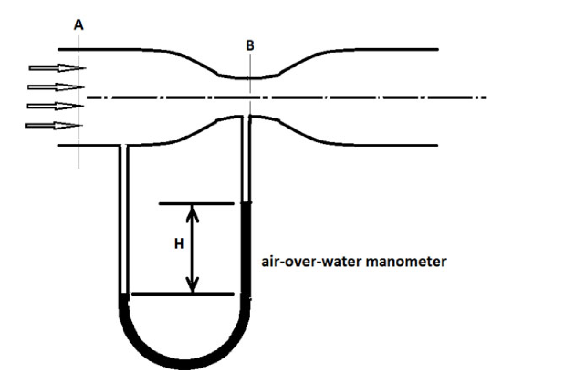
\includegraphics[width=0.5\linewidth]{figs/image8''.png}
    \caption{Caption}
    \label{fig:placeholder}
\end{figure}
\hfill(GATE MT 2020)


\item For effective comminution in a ball mill, it is desired that the balls travelling along the mill wall leave the wall at point C and travel freely in air along the path $CDA$, as shown in the figure. If $\angle BOC = 120^\circ$, the rotational speed of the mill is $\_\_\_\_\_$ rpm (rounded off to one decimal place) by performing suitable force balance at point C.  

\textbf{Assume:}  
\begin{enumerate}
\item There is no slip between the ball and mill wall.  
\item $O$ is the rotational axis of the mill and $OB$ is parallel to the vector $\mathbf{g}$.  
\item Inner diameter of ball mill is $3.26 \ \text{m}$.  
\item Acceleration due to gravity is $9.8 \ \text{m s}^{-2}$.  
\end{enumerate}

\begin{figure}[h]
    \centering
    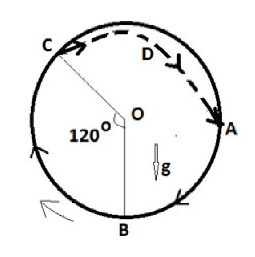
\includegraphics[width=0.5\linewidth]{figs/image9''.png}
    \caption{}
    \label{fig:placeholder}
\end{figure}
\hfill(GATE MT 2020)


\item If liquid copper is cooled to $1353 \ \text{K}$, magnitude of the driving force for liquid to transform to solid is $\_\_\_\_\_$ J.mol$^{-1}$ (round off to one decimal place).  

Given, melting temperature and enthalpy of melting of copper are $1356 \ \text{K}$ and $13 \ \text{kJ.mol}^{-1}$ respectively.  
\hfill(GATE MT 2020)


\item $1000 \ \text{kg}$ of liquid steel containing $0.03 \ \text{wt.\%}$ S needs to be desulphurized using a slag to bring the sulphur content down to $0.015 \ \text{wt.\%}$. The quantity of slag needed is $\_\_\_\_\_$ kg (round off to the nearest integer).  

\textbf{Assume:}  
\begin{enumerate}
\item Thermodynamic equilibrium.  
\item No sulphur in the slag prior to desulphurization treatment.  
\end{enumerate}

Given the equilibrium sulphur partition ratio between slag and steel,  
$$
\frac{\text{(wt.\% S)}_{\text{in slag}}}{\text{(wt.\% S)}_{\text{in steel}}} = 50
$$
\hfill(GATE MT 2020)


\item Zone refining of Si results in residual P content of $0.1$ parts per billion by weight. The electrical conductivity of this zone refined Si is $\_\_\_\_\_$ $\Omega^{-1}\text{m}^{-1}$ (round off to two decimal places).  

\textbf{Given:}  
\begin{itemize}
\item Avogadro number is $6.02 \times 10^{23}$.  
\item Density of Si is $2.33 \ \text{g cm}^{-3}$.  
\item Atomic weight of P is $30.97$.  
\item Charge of electron is $1.6 \times 10^{-19} \ \text{A.s}$.  
\item Mobility of electron is $0.2 \ \text{m}^2 \text{V}^{-1} \text{s}^{-1}$.  
\end{itemize}
\hfill(GATE MT 2020)


\item The steady state creep rate of a material increases by a factor of 20 when the temperature is increased from $890 \ \text{K}$ to $980 \ \text{K}$. The creep rate at a temperature of $\_\_\_\_\_$ K (round off to the nearest integer) will be 5 times the creep rate at $890 \ \text{K}$.  
\hfill(GATE MT 2020)


\item Crack growth is being continuously measured in a test specimen subjected to constant amplitude cyclic stress with a mean stress of zero. The crack growth rate is related to the stress intensity range, $\Delta K$, as  

$$
\frac{da}{dN} \propto \brak{\Delta K}^m
$$

where, $a$ is the crack length and $N$ is the number of cycles. When the crack length increases by a factor of two, the crack growth rate will increase by a factor of $\_\_\_\_\_$ (round off to one decimal place).  
\hfill(GATE MT 2020)


\item In a top gated mold, liquid metal enters the mold cavity as a freely falling stream under gravity from a height of $0.5 \ \text{m}$. Ignore the fluid friction due to viscosity and the drag due to changes in the direction of flow. If the volume of the mold cavity is $10 \ \text{m}^3$, then the time required to fill the mold is $\_\_\_\_\_$ s (round off to nearest integer).  

\textbf{Given:}  
\begin{enumerate}
\item Acceleration due to gravity is $9.8 \ \text{m.s}^{-2}$.  
\item Cross-sectional area of gate is $0.2 \ \text{m}^2$.  
\end{enumerate}
\hfill(GATE MT 2020)


\item A Basic Oxygen Furnace operator, at the end of oxygen blow, measures the dissolved oxygen content in the steel as $0.03 \ \text{wt.\%}$ and the steel temperature as $1800 \ \text{K}$. The carbon content [C] in the steel is $\_\_\_\_\_$ wt.\% (round off to two decimal places).  

\textbf{Assume:}  
\begin{enumerate}
\item Equilibrium between dissolved carbon \sbrak{C}, dissolved oxygen \sbrak{O}, and CO \brak{gas} at 1 atmosphere.  
\item Henry\textquotesingle s law is valid for both \sbrak{C} and \sbrak{O}.  
\end{enumerate}

\textbf{Given:}  

$$
[C]_{{1 \ wt.\% \ Henrian \ Std.\ State}} + [O]_{{1 \ wt.\% \ Henrian \ Std.\ State}} \rightarrow (CO)_{1 \ atm. \ Std.\ State}
$$

$$
\Delta G^\circ = -19840 - 40.65 \, T \ \text{J}
$$

$$
R = 8.314 \ \text{J.mol}^{-1} \text{K}^{-1}
$$
\hfill(GATE MT 2020)


\item $M$ and $N$ are $3 \times 3$ matrices. If $\det(M) = -9$ and $\det(N) = -14$, then the $\det(NM)$ is $\_\_\_\_\_$ (round off to the nearest integer).  
\hfill(GATE MT 2020)

\end{enumerate}

\end{document}